% Options for packages loaded elsewhere
\PassOptionsToPackage{unicode}{hyperref}
\PassOptionsToPackage{hyphens}{url}
%
\documentclass[
]{article}
\usepackage{amsmath,amssymb}
\usepackage{iftex}
\ifPDFTeX
  \usepackage[T1]{fontenc}
  \usepackage[utf8]{inputenc}
  \usepackage{textcomp} % provide euro and other symbols
\else % if luatex or xetex
  \usepackage{unicode-math} % this also loads fontspec
  \defaultfontfeatures{Scale=MatchLowercase}
  \defaultfontfeatures[\rmfamily]{Ligatures=TeX,Scale=1}
\fi
\usepackage{lmodern}
\ifPDFTeX\else
  % xetex/luatex font selection
\fi
% Use upquote if available, for straight quotes in verbatim environments
\IfFileExists{upquote.sty}{\usepackage{upquote}}{}
\IfFileExists{microtype.sty}{% use microtype if available
  \usepackage[]{microtype}
  \UseMicrotypeSet[protrusion]{basicmath} % disable protrusion for tt fonts
}{}
\makeatletter
\@ifundefined{KOMAClassName}{% if non-KOMA class
  \IfFileExists{parskip.sty}{%
    \usepackage{parskip}
  }{% else
    \setlength{\parindent}{0pt}
    \setlength{\parskip}{6pt plus 2pt minus 1pt}}
}{% if KOMA class
  \KOMAoptions{parskip=half}}
\makeatother
\usepackage{xcolor}
\usepackage[margin=1in]{geometry}
\usepackage{color}
\usepackage{fancyvrb}
\newcommand{\VerbBar}{|}
\newcommand{\VERB}{\Verb[commandchars=\\\{\}]}
\DefineVerbatimEnvironment{Highlighting}{Verbatim}{commandchars=\\\{\}}
% Add ',fontsize=\small' for more characters per line
\usepackage{framed}
\definecolor{shadecolor}{RGB}{248,248,248}
\newenvironment{Shaded}{\begin{snugshade}}{\end{snugshade}}
\newcommand{\AlertTok}[1]{\textcolor[rgb]{0.94,0.16,0.16}{#1}}
\newcommand{\AnnotationTok}[1]{\textcolor[rgb]{0.56,0.35,0.01}{\textbf{\textit{#1}}}}
\newcommand{\AttributeTok}[1]{\textcolor[rgb]{0.13,0.29,0.53}{#1}}
\newcommand{\BaseNTok}[1]{\textcolor[rgb]{0.00,0.00,0.81}{#1}}
\newcommand{\BuiltInTok}[1]{#1}
\newcommand{\CharTok}[1]{\textcolor[rgb]{0.31,0.60,0.02}{#1}}
\newcommand{\CommentTok}[1]{\textcolor[rgb]{0.56,0.35,0.01}{\textit{#1}}}
\newcommand{\CommentVarTok}[1]{\textcolor[rgb]{0.56,0.35,0.01}{\textbf{\textit{#1}}}}
\newcommand{\ConstantTok}[1]{\textcolor[rgb]{0.56,0.35,0.01}{#1}}
\newcommand{\ControlFlowTok}[1]{\textcolor[rgb]{0.13,0.29,0.53}{\textbf{#1}}}
\newcommand{\DataTypeTok}[1]{\textcolor[rgb]{0.13,0.29,0.53}{#1}}
\newcommand{\DecValTok}[1]{\textcolor[rgb]{0.00,0.00,0.81}{#1}}
\newcommand{\DocumentationTok}[1]{\textcolor[rgb]{0.56,0.35,0.01}{\textbf{\textit{#1}}}}
\newcommand{\ErrorTok}[1]{\textcolor[rgb]{0.64,0.00,0.00}{\textbf{#1}}}
\newcommand{\ExtensionTok}[1]{#1}
\newcommand{\FloatTok}[1]{\textcolor[rgb]{0.00,0.00,0.81}{#1}}
\newcommand{\FunctionTok}[1]{\textcolor[rgb]{0.13,0.29,0.53}{\textbf{#1}}}
\newcommand{\ImportTok}[1]{#1}
\newcommand{\InformationTok}[1]{\textcolor[rgb]{0.56,0.35,0.01}{\textbf{\textit{#1}}}}
\newcommand{\KeywordTok}[1]{\textcolor[rgb]{0.13,0.29,0.53}{\textbf{#1}}}
\newcommand{\NormalTok}[1]{#1}
\newcommand{\OperatorTok}[1]{\textcolor[rgb]{0.81,0.36,0.00}{\textbf{#1}}}
\newcommand{\OtherTok}[1]{\textcolor[rgb]{0.56,0.35,0.01}{#1}}
\newcommand{\PreprocessorTok}[1]{\textcolor[rgb]{0.56,0.35,0.01}{\textit{#1}}}
\newcommand{\RegionMarkerTok}[1]{#1}
\newcommand{\SpecialCharTok}[1]{\textcolor[rgb]{0.81,0.36,0.00}{\textbf{#1}}}
\newcommand{\SpecialStringTok}[1]{\textcolor[rgb]{0.31,0.60,0.02}{#1}}
\newcommand{\StringTok}[1]{\textcolor[rgb]{0.31,0.60,0.02}{#1}}
\newcommand{\VariableTok}[1]{\textcolor[rgb]{0.00,0.00,0.00}{#1}}
\newcommand{\VerbatimStringTok}[1]{\textcolor[rgb]{0.31,0.60,0.02}{#1}}
\newcommand{\WarningTok}[1]{\textcolor[rgb]{0.56,0.35,0.01}{\textbf{\textit{#1}}}}
\usepackage{graphicx}
\makeatletter
\def\maxwidth{\ifdim\Gin@nat@width>\linewidth\linewidth\else\Gin@nat@width\fi}
\def\maxheight{\ifdim\Gin@nat@height>\textheight\textheight\else\Gin@nat@height\fi}
\makeatother
% Scale images if necessary, so that they will not overflow the page
% margins by default, and it is still possible to overwrite the defaults
% using explicit options in \includegraphics[width, height, ...]{}
\setkeys{Gin}{width=\maxwidth,height=\maxheight,keepaspectratio}
% Set default figure placement to htbp
\makeatletter
\def\fps@figure{htbp}
\makeatother
\setlength{\emergencystretch}{3em} % prevent overfull lines
\providecommand{\tightlist}{%
  \setlength{\itemsep}{0pt}\setlength{\parskip}{0pt}}
\setcounter{secnumdepth}{-\maxdimen} % remove section numbering
\usepackage{hyperref}
\hypersetup{colorlinks=true, linkcolor=red, urlcolor=blue}
\ifLuaTeX
  \usepackage{selnolig}  % disable illegal ligatures
\fi
\IfFileExists{bookmark.sty}{\usepackage{bookmark}}{\usepackage{hyperref}}
\IfFileExists{xurl.sty}{\usepackage{xurl}}{} % add URL line breaks if available
\urlstyle{same}
\hypersetup{
  pdftitle={(Fast) Introduction to R},
  pdfauthor={Joana Cima},
  hidelinks,
  pdfcreator={LaTeX via pandoc}}

\title{(Fast) Introduction to R}
\usepackage{etoolbox}
\makeatletter
\providecommand{\subtitle}[1]{% add subtitle to \maketitle
  \apptocmd{\@title}{\par {\large #1 \par}}{}{}
}
\makeatother
\subtitle{Jump into a notebook}
\author{Joana Cima}
\date{05 dezembro 2023}

\begin{document}
\maketitle

\hypertarget{my-beamer}{%
\section{My beamer}\label{my-beamer}}

\begin{quote}
BlaBlaBla
\end{quote}

\hypertarget{outline}{%
\section{Outline}\label{outline}}

\begin{enumerate}
\def\labelenumi{\arabic{enumi}.}
\tightlist
\item
  Motivation
\item
  Data
\item
  Conceptual discussion
\end{enumerate}

\hypertarget{import-data-from-an-excel-file}{%
\section{3. Import data (from an excel
file)}\label{import-data-from-an-excel-file}}

\hypertarget{load-your-data-using-point-and-click}{%
\subsection{Load your data using point and
click}\label{load-your-data-using-point-and-click}}

\begin{figure}
\centering
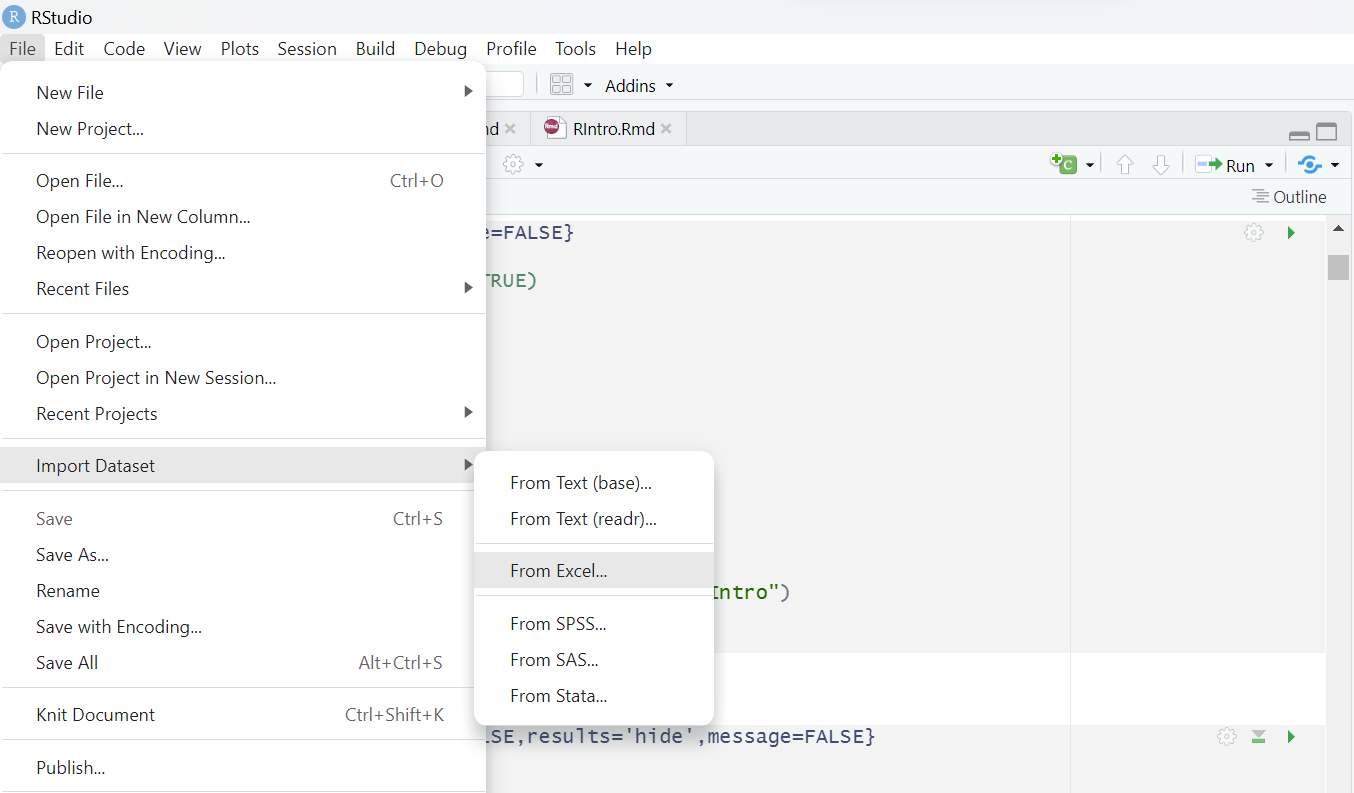
\includegraphics[width=0.31\textwidth,height=\textheight]{importdataset.png}
\caption{Point and click}
\end{figure}

which corresponds to the following code

\begin{Shaded}
\begin{Highlighting}[]
\NormalTok{nlswork }\OtherTok{\textless{}{-}} \FunctionTok{as.data.frame}\NormalTok{(}\FunctionTok{read\_excel}\NormalTok{(}\StringTok{"nlswork.xlsx"}\NormalTok{))}
\CommentTok{\# nlswork \textless{}{-} read\_dta("nlswork.dta") \# in case you have a Stata data source}

\FunctionTok{head}\NormalTok{(nlswork)}
\end{Highlighting}
\end{Shaded}

\begin{verbatim}
##   idcode year birth_yr age  race msp nev_mar grade collgrad not_smsa c_city
## 1      1   70       51  18 black   0       1    12        0        0      1
## 2      1   71       51  19 black   1       0    12        0        0      1
## 3      1   72       51  20 black   1       0    12        0        0      1
## 4      1   73       51  21 black   1       0    12        0        0      1
## 5      1   75       51  23 black   1       0    12        0        0      1
## 6      1   77       51  25 black   0       0    12        0        0      1
##   south ind_code occ_code union wks_ue  ttl_exp     tenure hours wks_work
## 1     0        6        3    NA      2 1.083333 0.08333334    20       27
## 2     0        4        6    NA     22 1.275641 0.08333334    44       10
## 3     0        4        6     1      0 2.256410 0.91666669    40       51
## 4     0        4        6    NA      0 2.314102 0.08333334    40        3
## 5     0        5        6    NA      0 2.775641 0.16666667    10       24
## 6     0       12        8     0      0 3.775641 1.50000000    32       52
##    ln_wage
## 1 1.451214
## 2 1.028620
## 3 1.589977
## 4 1.780273
## 5 1.777012
## 6 1.778681
\end{verbatim}

\begin{Shaded}
\begin{Highlighting}[]
\FunctionTok{colnames}\NormalTok{(nlswork)}
\end{Highlighting}
\end{Shaded}

\begin{verbatim}
##  [1] "idcode"   "year"     "birth_yr" "age"      "race"     "msp"     
##  [7] "nev_mar"  "grade"    "collgrad" "not_smsa" "c_city"   "south"   
## [13] "ind_code" "occ_code" "union"    "wks_ue"   "ttl_exp"  "tenure"  
## [19] "hours"    "wks_work" "ln_wage"
\end{verbatim}

\begin{Shaded}
\begin{Highlighting}[]
\FunctionTok{str}\NormalTok{(nlswork)}
\end{Highlighting}
\end{Shaded}

\begin{verbatim}
## 'data.frame':    28534 obs. of  21 variables:
##  $ idcode  : num  1 1 1 1 1 1 1 1 1 1 ...
##  $ year    : num  70 71 72 73 75 77 78 80 83 85 ...
##  $ birth_yr: num  51 51 51 51 51 51 51 51 51 51 ...
##  $ age     : num  18 19 20 21 23 25 26 28 31 33 ...
##  $ race    : chr  "black" "black" "black" "black" ...
##  $ msp     : num  0 1 1 1 1 0 0 0 0 0 ...
##  $ nev_mar : num  1 0 0 0 0 0 0 0 0 0 ...
##  $ grade   : num  12 12 12 12 12 12 12 12 12 12 ...
##  $ collgrad: num  0 0 0 0 0 0 0 0 0 0 ...
##  $ not_smsa: num  0 0 0 0 0 0 0 0 0 0 ...
##  $ c_city  : num  1 1 1 1 1 1 1 1 1 1 ...
##  $ south   : num  0 0 0 0 0 0 0 0 0 0 ...
##  $ ind_code: num  6 4 4 4 5 12 5 5 5 5 ...
##  $ occ_code: num  3 6 6 6 6 8 6 6 6 6 ...
##  $ union   : num  NA NA 1 NA NA 0 NA 1 1 1 ...
##  $ wks_ue  : num  2 22 0 0 0 0 7 0 NA 0 ...
##  $ ttl_exp : num  1.08 1.28 2.26 2.31 2.78 ...
##  $ tenure  : num  0.0833 0.0833 0.9167 0.0833 0.1667 ...
##  $ hours   : num  20 44 40 40 10 32 52 45 49 42 ...
##  $ wks_work: num  27 10 51 3 24 52 4 75 101 97 ...
##  $ ln_wage : num  1.45 1.03 1.59 1.78 1.78 ...
\end{verbatim}

\hypertarget{data-manipulation-check-the-pipe-operator}{%
\section{4. Data manipulation -- check the pipe operator,
\%\textgreater\%}\label{data-manipulation-check-the-pipe-operator}}

\hypertarget{select-a-subset-of-variables}{%
\subsection{4.1. Select a subset of
variables}\label{select-a-subset-of-variables}}

\begin{Shaded}
\begin{Highlighting}[]
\NormalTok{nlswork\_s}\OtherTok{\textless{}{-}}\NormalTok{ nlswork }\SpecialCharTok{\%\textgreater{}\%} 
  \FunctionTok{select}\NormalTok{(idcode, ln\_wage) }
\end{Highlighting}
\end{Shaded}

\hypertarget{rename-variables}{%
\subsection{4.2. Rename variables}\label{rename-variables}}

\begin{Shaded}
\begin{Highlighting}[]
\NormalTok{nlswork\_r }\OtherTok{\textless{}{-}}\NormalTok{ nlswork }\SpecialCharTok{\%\textgreater{}\%} 
  \FunctionTok{rename}\NormalTok{(}\AttributeTok{cae =}\NormalTok{ ind\_code)}
\end{Highlighting}
\end{Shaded}

\hypertarget{filter-a-subset-of-observations}{%
\subsection{4.3. Filter a subset of
observations}\label{filter-a-subset-of-observations}}

\begin{Shaded}
\begin{Highlighting}[]
\NormalTok{nlswork\_f}\OtherTok{\textless{}{-}}\NormalTok{ nlswork }\SpecialCharTok{\%\textgreater{}\%} 
  \FunctionTok{filter}\NormalTok{(age }\SpecialCharTok{\textgreater{}} \DecValTok{20}\NormalTok{) }
\end{Highlighting}
\end{Shaded}

\hypertarget{mutate-create-variables}{%
\subsection{4.4. Mutate: create
variables}\label{mutate-create-variables}}

\begin{Shaded}
\begin{Highlighting}[]
\NormalTok{ nlswork\_m }\OtherTok{\textless{}{-}}\NormalTok{ nlswork }\SpecialCharTok{\%\textgreater{}\%} 
  \FunctionTok{mutate}\NormalTok{(}\AttributeTok{ln\_asd=}\FunctionTok{log}\NormalTok{(age))}
\end{Highlighting}
\end{Shaded}

\hypertarget{manipulate-the-data-in-a-single-sequence}{%
\subsection{4.5. Manipulate the data in a single
sequence}\label{manipulate-the-data-in-a-single-sequence}}

\begin{Shaded}
\begin{Highlighting}[]
\NormalTok{nlswork\_new }\OtherTok{\textless{}{-}}\NormalTok{ nlswork }\SpecialCharTok{\%\textgreater{}\%} 
  \FunctionTok{rename}\NormalTok{(}\AttributeTok{cae =}\NormalTok{ ind\_code) }\SpecialCharTok{\%\textgreater{}\%}
  \FunctionTok{select}\NormalTok{(ln\_wage, age, year, race, union, collgrad, cae, ttl\_exp, hours ) }\SpecialCharTok{\%\textgreater{}\%} 
  \FunctionTok{filter}\NormalTok{(age}\SpecialCharTok{\textgreater{}=}\DecValTok{20}\NormalTok{) }\SpecialCharTok{\%\textgreater{}\%}
  \FunctionTok{mutate}\NormalTok{(}\AttributeTok{age2=}\NormalTok{age}\SpecialCharTok{\^{}}\DecValTok{2}\NormalTok{)}
\end{Highlighting}
\end{Shaded}

\hypertarget{detecting-and-handling-missing-data}{%
\section{5. Detecting and Handling Missing
Data}\label{detecting-and-handling-missing-data}}

\hypertarget{detect-missing-data}{%
\subsection{5.1 Detect Missing Data}\label{detect-missing-data}}

\begin{Shaded}
\begin{Highlighting}[]
\FunctionTok{vis\_miss}\NormalTok{(nlswork\_new)}
\end{Highlighting}
\end{Shaded}

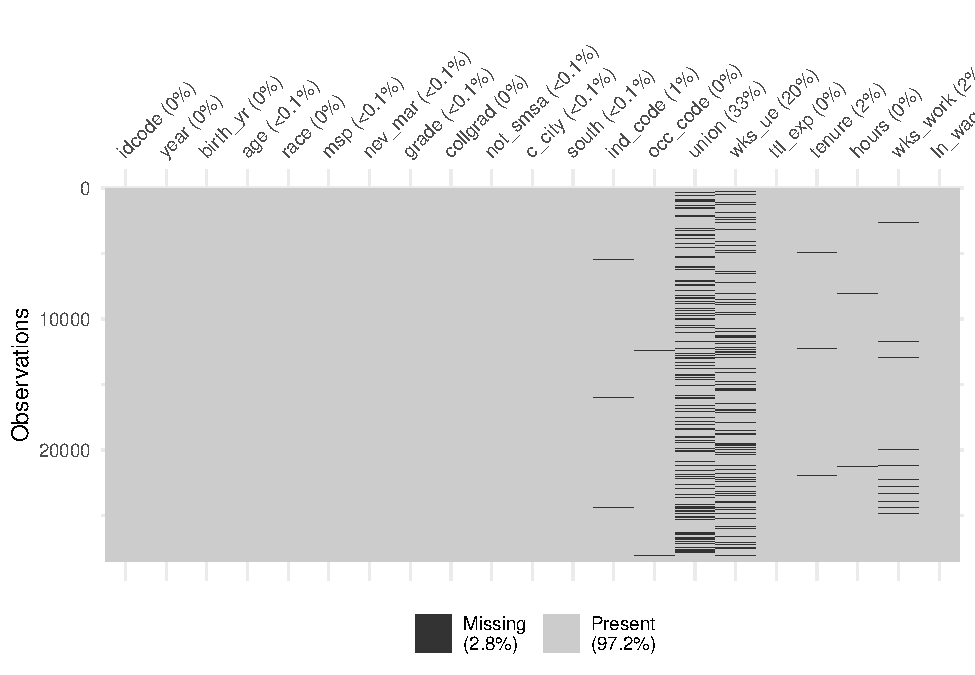
\includegraphics{RIntro_files/figure-latex/unnamed-chunk-7-1.pdf}

\begin{Shaded}
\begin{Highlighting}[]
\FunctionTok{gg\_miss\_var}\NormalTok{(nlswork\_new) }\SpecialCharTok{+} \FunctionTok{labs}\NormalTok{(}\AttributeTok{y =} \StringTok{"Total missing values for each variable"}\NormalTok{)}
\end{Highlighting}
\end{Shaded}

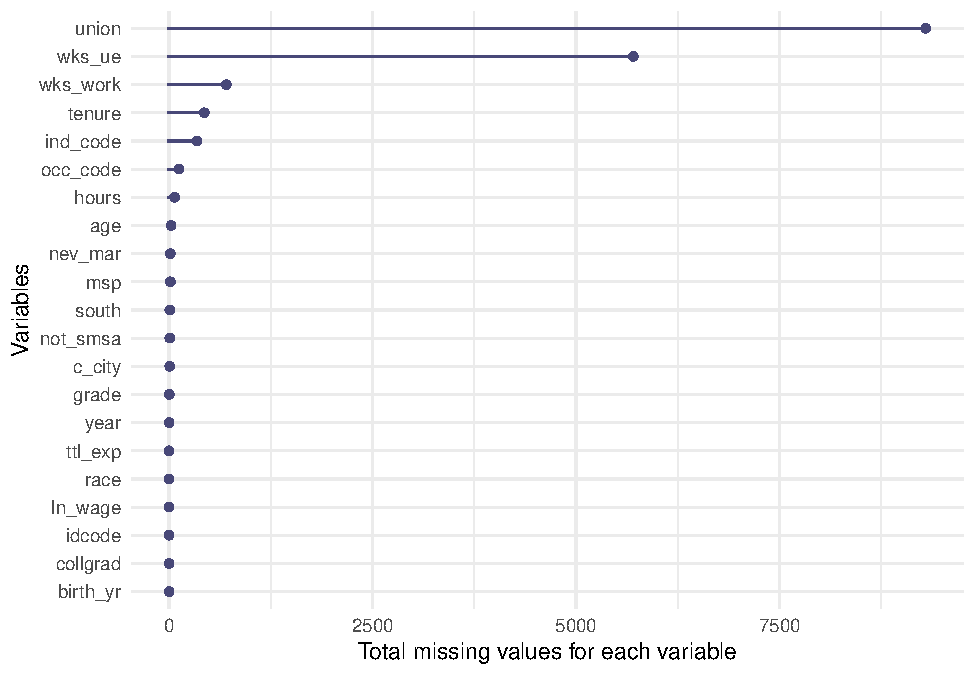
\includegraphics{RIntro_files/figure-latex/unnamed-chunk-8-1.pdf}

\begin{Shaded}
\begin{Highlighting}[]
\FunctionTok{gg\_miss\_upset}\NormalTok{(nlswork\_new)}
\end{Highlighting}
\end{Shaded}

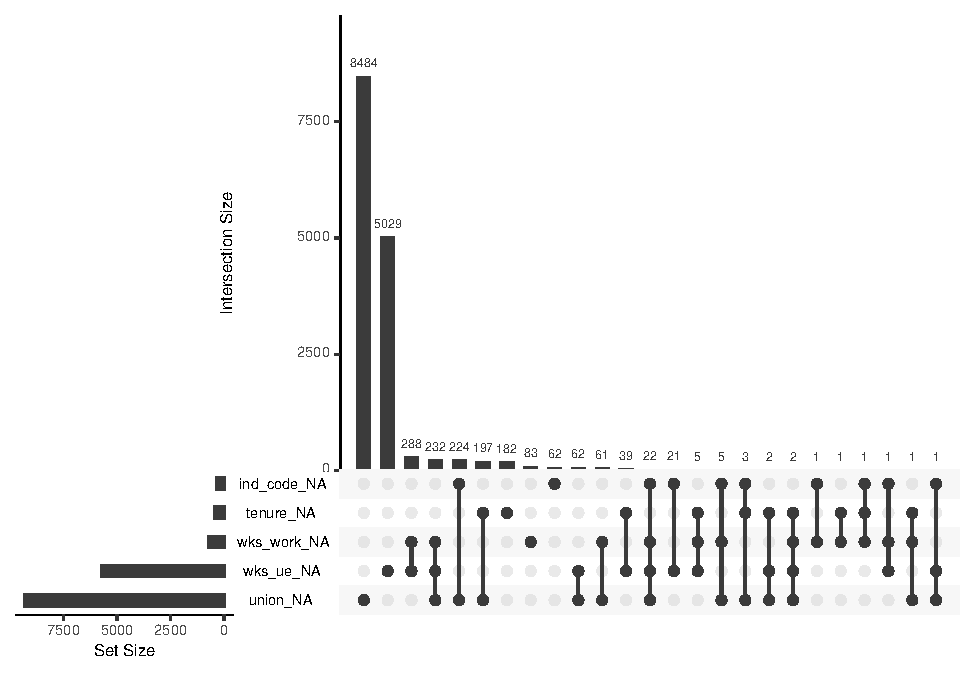
\includegraphics{RIntro_files/figure-latex/unnamed-chunk-8-2.pdf}

\begin{Shaded}
\begin{Highlighting}[]
\FunctionTok{gg\_miss\_fct}\NormalTok{(}\AttributeTok{x =}\NormalTok{ nlswork\_new,}\AttributeTok{fct =}\NormalTok{ year)}
\end{Highlighting}
\end{Shaded}

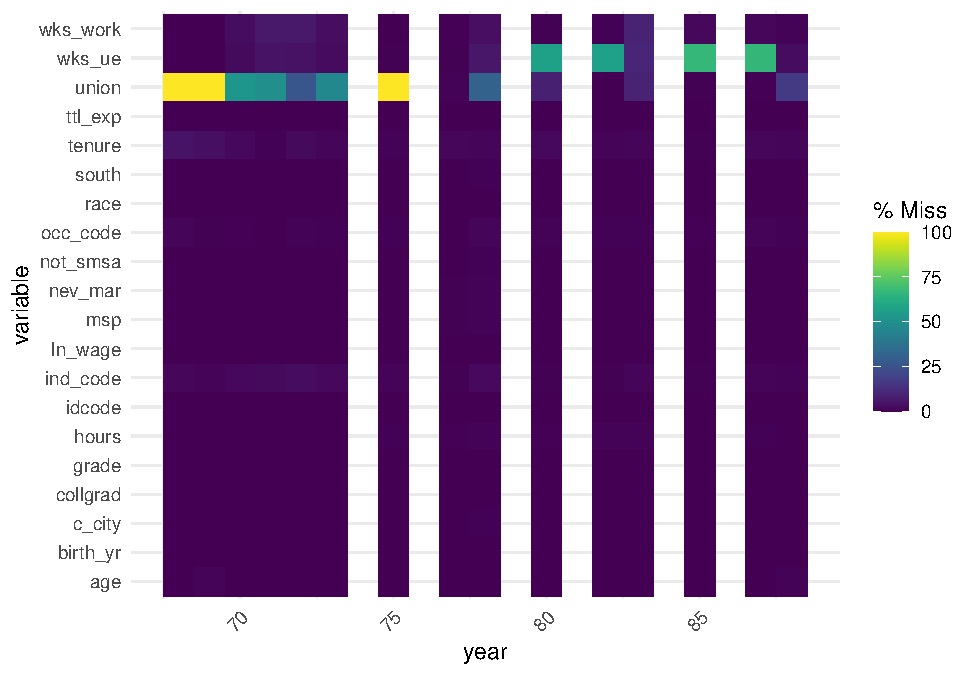
\includegraphics{RIntro_files/figure-latex/unnamed-chunk-9-1.pdf}

\hypertarget{alternative}{%
\subsubsection{Alternative}\label{alternative}}

\begin{Shaded}
\begin{Highlighting}[]
\FunctionTok{vis\_dat}\NormalTok{(nlswork\_new)}
\end{Highlighting}
\end{Shaded}

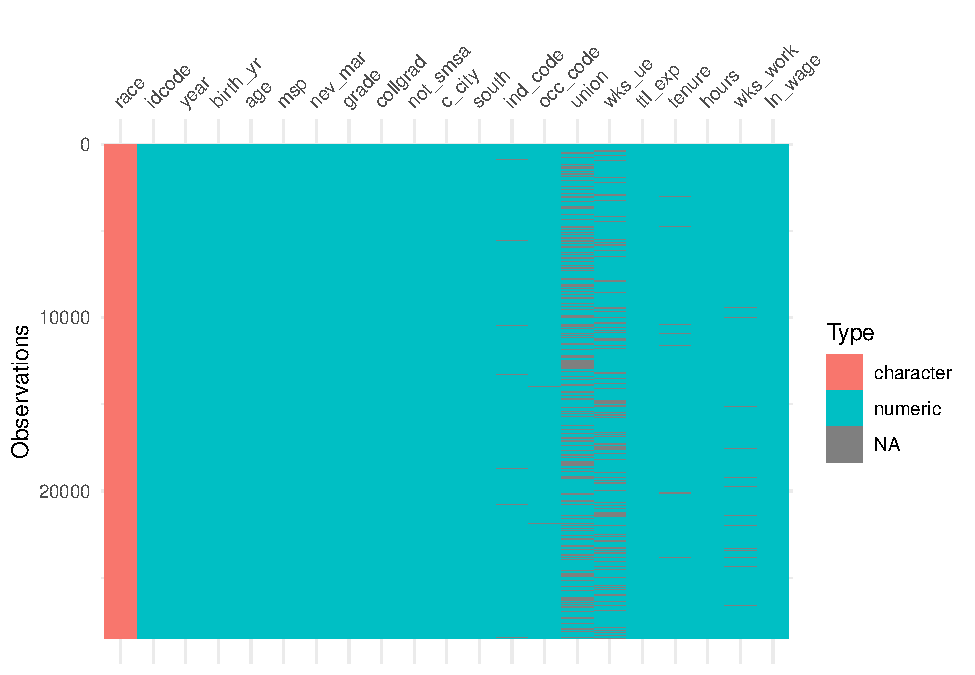
\includegraphics{RIntro_files/figure-latex/unnamed-chunk-10-1.pdf}

\hypertarget{handling-missing-data}{%
\subsection{5.2. Handling Missing Data}\label{handling-missing-data}}

Handling missing data is a crucial step in the exploratory data
analysis. Depending on the nature and mechanism of the missingness, we
might decide to impute missing values or to exclude the observations
with missing data.

\hypertarget{filling-missing-data}{%
\subsubsection{5.2.1 Filling Missing Data}\label{filling-missing-data}}

In some situations, we may opt to fill in the missing data. For
instance, one common method involves replacing missing values with the
mean of the variable.

\begin{Shaded}
\begin{Highlighting}[]
\FunctionTok{library}\NormalTok{(tidyverse)}
\CommentTok{\# Filling Missing Data }

\DocumentationTok{\#\# (with the average {-} this is an example {-} it does not make sense in this case)}
\NormalTok{nlswork\_filled }\OtherTok{\textless{}{-}}\NormalTok{ nlswork }\SpecialCharTok{\%\textgreater{}\%} 
  \FunctionTok{mutate}\NormalTok{(}\FunctionTok{across}\NormalTok{(}\FunctionTok{c}\NormalTok{(}\StringTok{"union"}\NormalTok{), }\SpecialCharTok{\textasciitilde{}} \FunctionTok{ifelse}\NormalTok{(}\FunctionTok{is.na}\NormalTok{(.), }\FunctionTok{mean}\NormalTok{(., }\AttributeTok{na.rm =} \ConstantTok{TRUE}\NormalTok{), .))) }

\DocumentationTok{\#\# (with the mode)}
    \DocumentationTok{\#\#\# Create a function to compute mode}

\NormalTok{mode }\OtherTok{\textless{}{-}} \ControlFlowTok{function}\NormalTok{(x) \{}
\NormalTok{  ux }\OtherTok{\textless{}{-}} \FunctionTok{unique}\NormalTok{(x)}
\NormalTok{  ux[}\FunctionTok{which.max}\NormalTok{(}\FunctionTok{tabulate}\NormalTok{(}\FunctionTok{match}\NormalTok{(x, ux)))]}
\NormalTok{\}}

\NormalTok{nlswork\_filled2 }\OtherTok{\textless{}{-}}\NormalTok{ nlswork}

\NormalTok{union\_mode }\OtherTok{\textless{}{-}} \FunctionTok{mode}\NormalTok{(nlswork}\SpecialCharTok{$}\NormalTok{union[}\SpecialCharTok{!}\FunctionTok{is.na}\NormalTok{(nlswork}\SpecialCharTok{$}\NormalTok{union)])}
\NormalTok{nlswork\_filled2}\SpecialCharTok{$}\NormalTok{union[}\FunctionTok{is.na}\NormalTok{(nlswork}\SpecialCharTok{$}\NormalTok{union)] }\OtherTok{\textless{}{-}}\NormalTok{ union\_mode}
\end{Highlighting}
\end{Shaded}

\hypertarget{excluding-rows-with-missing-data}{%
\subsubsection{5.2.2 Excluding rows with missing
data}\label{excluding-rows-with-missing-data}}

\begin{Shaded}
\begin{Highlighting}[]
\NormalTok{nlswork\_no\_na }\OtherTok{\textless{}{-}} \FunctionTok{na.omit}\NormalTok{(nlswork\_new)}
\end{Highlighting}
\end{Shaded}

\hypertarget{detecting-and-handling-outliers}{%
\section{6 Detecting and Handling
Outliers}\label{detecting-and-handling-outliers}}

\hypertarget{detecting-outliers}{%
\subsection{6.1 Detecting Outliers}\label{detecting-outliers}}

\hypertarget{using-boxplot-example-age-and-ln_wage}{%
\subsubsection{6.1.1. Using Boxplot (example: age and
ln\_wage)}\label{using-boxplot-example-age-and-ln_wage}}

\begin{Shaded}
\begin{Highlighting}[]
\FunctionTok{boxplot}\NormalTok{(nlswork\_no\_na}\SpecialCharTok{$}\NormalTok{age, }\AttributeTok{main=}\StringTok{"Boxplot for Outlier Detection {-} Age"}\NormalTok{)}
\end{Highlighting}
\end{Shaded}

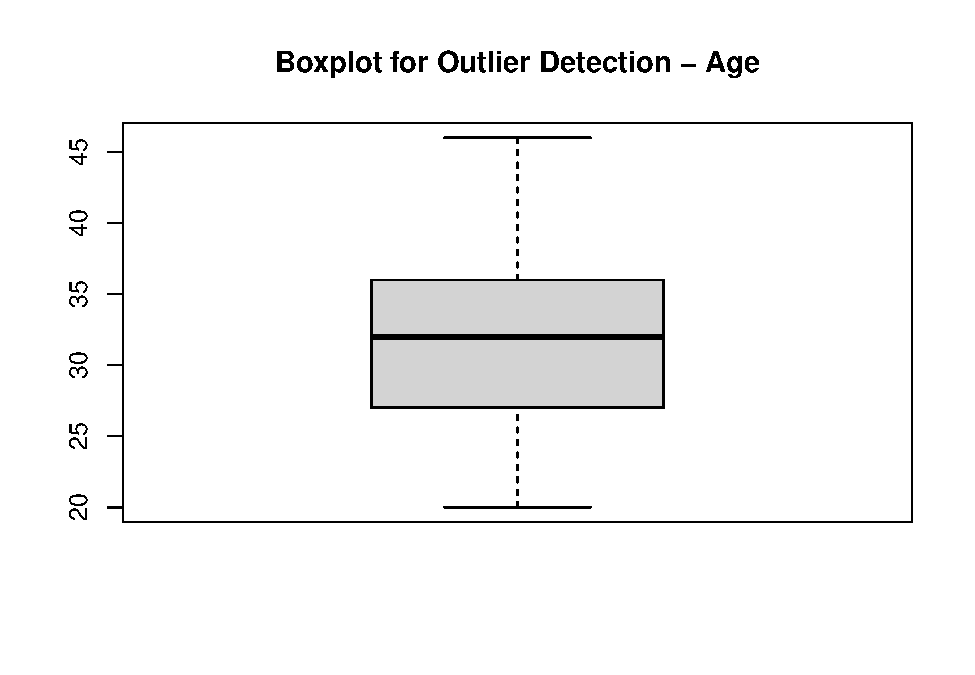
\includegraphics{RIntro_files/figure-latex/unnamed-chunk-13-1.pdf}

\begin{Shaded}
\begin{Highlighting}[]
\FunctionTok{boxplot}\NormalTok{(nlswork\_no\_na}\SpecialCharTok{$}\NormalTok{ln\_wage, }\AttributeTok{main=}\StringTok{"Boxplot for Outlier Detection {-} ln\_wage"}\NormalTok{)}
\end{Highlighting}
\end{Shaded}

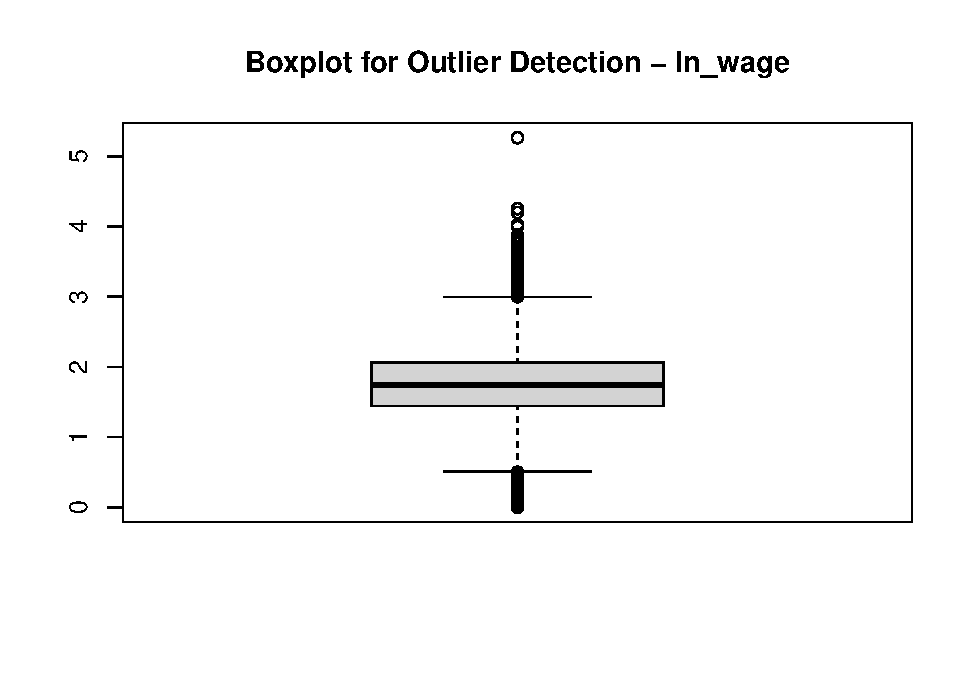
\includegraphics{RIntro_files/figure-latex/unnamed-chunk-14-1.pdf}
\#\#\# 6.1.2. Detecting Outliers using ``identify\_outliers'' (example:
ln\_wage)

\begin{Shaded}
\begin{Highlighting}[]
\NormalTok{outliers }\OtherTok{\textless{}{-}} \FunctionTok{identify\_outliers}\NormalTok{(}\FunctionTok{as.data.frame}\NormalTok{(nlswork\_no\_na}\SpecialCharTok{$}\NormalTok{ln\_wage))}
\NormalTok{extreme\_outliers }\OtherTok{\textless{}{-}}\NormalTok{ outliers[outliers}\SpecialCharTok{$}\NormalTok{is.extreme, ]}
\NormalTok{extreme\_outliers}
\end{Highlighting}
\end{Shaded}

\begin{verbatim}
##     nlswork_no_na$ln_wage is.outlier is.extreme
## 73               4.025415       TRUE       TRUE
## 149              4.005049       TRUE       TRUE
## 159              5.263916       TRUE       TRUE
## 235              4.254619       TRUE       TRUE
## 249              3.997510       TRUE       TRUE
## 254              4.199647       TRUE       TRUE
\end{verbatim}

\hypertarget{handling-outliers}{%
\subsection{6.2 Handling Outliers}\label{handling-outliers}}

\hypertarget{removing-the-outliers-from-the-original-dataframe-nlswork_no_na}{%
\subsubsection{6.2.1 Removing the outliers from the original dataframe
nlswork\_no\_na}\label{removing-the-outliers-from-the-original-dataframe-nlswork_no_na}}

\begin{Shaded}
\begin{Highlighting}[]
\NormalTok{extreme\_values\_to\_remove }\OtherTok{\textless{}{-}}\NormalTok{ extreme\_outliers}\SpecialCharTok{$}\StringTok{\textasciigrave{}}\AttributeTok{nlswork\_no\_na$ln\_wage}\StringTok{\textasciigrave{}}
\NormalTok{nlswork\_no\_outliers }\OtherTok{\textless{}{-}}\NormalTok{ nlswork\_no\_na[}\SpecialCharTok{!}\NormalTok{nlswork\_no\_na}\SpecialCharTok{$}\NormalTok{ln\_wage }\SpecialCharTok{\%in\%}\NormalTok{ extreme\_values\_to\_remove, ]}
\end{Highlighting}
\end{Shaded}

\hypertarget{replacing-the-outliers-using-winsorize}{%
\subsubsection{6.2.2 Replacing the outliers using
winsorize}\label{replacing-the-outliers-using-winsorize}}

\begin{Shaded}
\begin{Highlighting}[]
\NormalTok{nlswork\_no\_na}\SpecialCharTok{$}\NormalTok{ln\_wage\_winsorized }\OtherTok{\textless{}{-}} \FunctionTok{Winsorize}\NormalTok{(nlswork\_no\_na}\SpecialCharTok{$}\NormalTok{ln\_wage, }
                                    \AttributeTok{probs =} \FunctionTok{c}\NormalTok{(}\DecValTok{0}\NormalTok{, }\FloatTok{0.99}\NormalTok{))}
\end{Highlighting}
\end{Shaded}

\hypertarget{descriptive-statistics}{%
\section{7. Descriptive statistics}\label{descriptive-statistics}}

\begin{Shaded}
\begin{Highlighting}[]
\FunctionTok{summary}\NormalTok{(nlswork\_no\_na) }
\end{Highlighting}
\end{Shaded}

\begin{verbatim}
##     ln_wage           age             year           race          
##  Min.   :0.000   Min.   :20.00   Min.   :70.00   Length:18703      
##  1st Qu.:1.442   1st Qu.:27.00   1st Qu.:77.00   Class :character  
##  Median :1.742   Median :32.00   Median :82.00   Mode  :character  
##  Mean   :1.763   Mean   :31.63   Mean   :80.57                     
##  3rd Qu.:2.065   3rd Qu.:36.00   3rd Qu.:85.00                     
##  Max.   :5.264   Max.   :46.00   Max.   :88.00                     
##      union           collgrad           cae            ttl_exp        
##  Min.   :0.0000   Min.   :0.0000   Min.   : 1.000   Min.   : 0.01923  
##  1st Qu.:0.0000   1st Qu.:0.0000   1st Qu.: 5.000   1st Qu.: 4.13462  
##  Median :0.0000   Median :0.0000   Median : 7.000   Median : 7.14103  
##  Mean   :0.2349   Mean   :0.1999   Mean   : 7.892   Mean   : 7.85462  
##  3rd Qu.:0.0000   3rd Qu.:0.0000   3rd Qu.:11.000   3rd Qu.:10.96795  
##  Max.   :1.0000   Max.   :1.0000   Max.   :12.000   Max.   :28.88462  
##      hours             age2      ln_wage_winsorized
##  Min.   :  1.00   Min.   : 400   Min.   :0.000     
##  1st Qu.: 35.00   1st Qu.: 729   1st Qu.:1.442     
##  Median : 40.00   Median :1024   Median :1.742     
##  Mean   : 36.77   Mean   :1036   Mean   :1.760     
##  3rd Qu.: 40.00   3rd Qu.:1296   3rd Qu.:2.065     
##  Max.   :168.00   Max.   :2116   Max.   :2.963
\end{verbatim}

\hypertarget{export-descriptive-statistics-table-to-html-with-2-digits}{%
\subsection{7.1. Export descriptive statistics table to html, with 2
digits}\label{export-descriptive-statistics-table-to-html-with-2-digits}}

\hypertarget{shorter-statistics}{%
\section{Shorter statistics}\label{shorter-statistics}}

\hypertarget{statistic-n-mean-st.-dev.-min-max}{%
\subsection{Statistic N Mean St.~Dev. Min
Max}\label{statistic-n-mean-st.-dev.-min-max}}

age 18,703 31.63 5.96 20 46\\
collgrad 18,703 0.20 0.40 0 1\\
ttl\_exp 18,703 7.85 4.54 0.02 28.88 union 18,703 0.23 0.42 0 1\\
hours 18,703 36.77 9.59 1 168 ln\_wage\_winsorized 18,703 1.76 0.46 0.00
2.96 ---------------------------------------------------

\hypertarget{export-descriptive-statistics-table-to-txt-with-3-digits}{%
\subsection{7.2. Export descriptive statistics table to txt, with 3
digits}\label{export-descriptive-statistics-table-to-txt-with-3-digits}}

\hypertarget{shorter-statistics-1}{%
\section{Shorter statistics}\label{shorter-statistics-1}}

\hypertarget{statistic-n-mean-st.-dev.-min-max-1}{%
\subsection{Statistic N Mean St.~Dev. Min
Max}\label{statistic-n-mean-st.-dev.-min-max-1}}

age 18,703 31.634 5.960 20 46\\
collgrad 18,703 0.200 0.400 0 1\\
ttl\_exp 18,703 7.855 4.536 0.019 28.885 union 18,703 0.235 0.424 0 1\\
hours 18,703 36.772 9.586 1 168\\
ln\_wage\_winsorized 18,703 1.760 0.458 0.000 2.963
------------------------------------------------------

\hypertarget{transposing-the-descriptive-statistics-table}{%
\subsection{7.3. Transposing the descriptive statistics
table}\label{transposing-the-descriptive-statistics-table}}

\hypertarget{shorter-statistics-2}{%
\section{Shorter statistics}\label{shorter-statistics-2}}

\hypertarget{statistic-age-collgrad-ttl_exp-union-hours-ln_wage_winsorized}{%
\subsection{Statistic age collgrad ttl\_exp union hours
ln\_wage\_winsorized}\label{statistic-age-collgrad-ttl_exp-union-hours-ln_wage_winsorized}}

N 18,703 18,703 18,703 18,703 18,703 18,703\\
Mean 31.634 0.200 7.855 0.235 36.772 1.760\\
St.~Dev. 5.960 0.400 4.536 0.424 9.586 0.458\\
Min 20 0 0.019 0 1 0.000\\
Max 46 1 28.885 1 168 2.963\\
------------------------------------------------------------------

\hypertarget{export-to-pdf}{%
\subsection{7.4. Export to pdf}\label{export-to-pdf}}

\% Table created by stargazer v.5.2.3 by Marek Hlavac, Social Policy
Institute. E-mail: marek.hlavac at gmail.com \% Date and time: ter, dez
05, 2023 - 22:05:41

\begin{table}[!htbp] \centering 
  \caption{Shorter statistics} 
  \label{} 
\begin{tabular}{@{\extracolsep{5pt}}lccccc} 
\\[-1.8ex]\hline 
\hline \\[-1.8ex] 
Statistic & age & collgrad & ttl\_exp & union & hours \\ 
\hline \\[-1.8ex] 
N & 18,703 & 18,703 & 18,703 & 18,703 & 18,703 \\ 
Mean & 31.634 & 0.200 & 7.855 & 0.235 & 36.772 \\ 
St. Dev. & 5.960 & 0.400 & 4.536 & 0.424 & 9.586 \\ 
Min & 20 & 0 & 0.019 & 0 & 1 \\ 
Max & 46 & 1 & 28.885 & 1 & 168 \\ 
\hline \\[-1.8ex] 
\end{tabular} 
\end{table}

\hypertarget{visualisation-to-explore-your-data}{%
\section{8. Visualisation to explore your
data}\label{visualisation-to-explore-your-data}}

\hypertarget{relationship-between-continuous-variables}{%
\subsection{8.1. Relationship Between Continuous
Variables}\label{relationship-between-continuous-variables}}

\begin{verbatim}
## `geom_smooth()` using formula = 'y ~ x'
\end{verbatim}

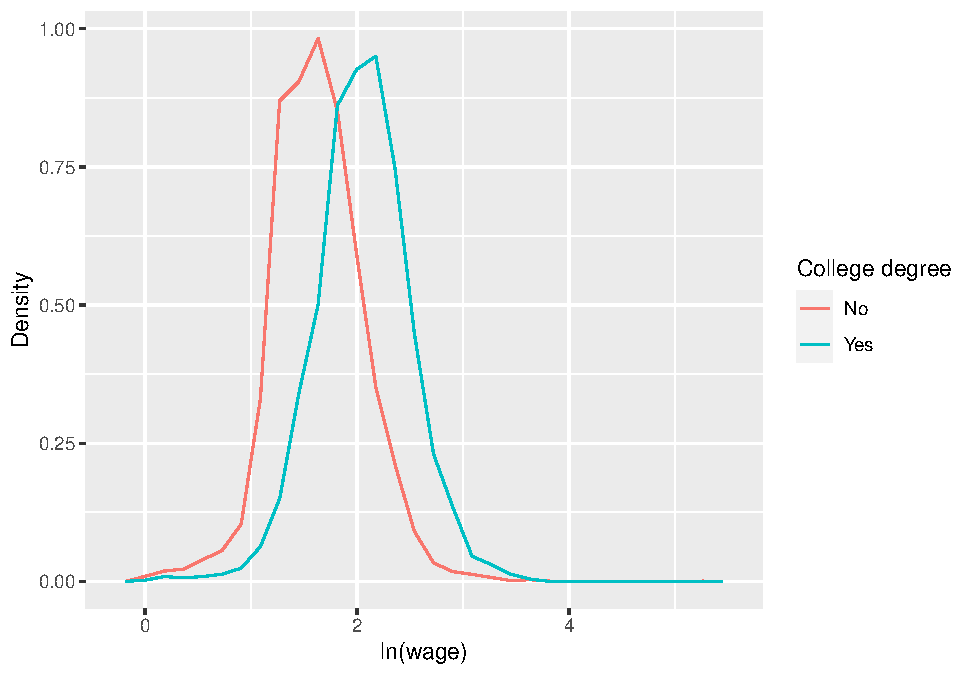
\includegraphics{RIntro_files/figure-latex/unnamed-chunk-23-1.pdf}

\hypertarget{categorical-variable}{%
\subsection{8.2. Categorical variable}\label{categorical-variable}}

\begin{Shaded}
\begin{Highlighting}[]
\FunctionTok{ggplot}\NormalTok{(}\AttributeTok{data =}\NormalTok{ nlswork\_no\_na) }\SpecialCharTok{+}
  \FunctionTok{geom\_bar}\NormalTok{(}\AttributeTok{mapping=}\FunctionTok{aes}\NormalTok{(}\AttributeTok{x=}\FunctionTok{as.factor}\NormalTok{(collgrad))) }\SpecialCharTok{+}
  \FunctionTok{xlab}\NormalTok{(}\StringTok{"College graduate (1=Yes)"}\NormalTok{)}
\end{Highlighting}
\end{Shaded}

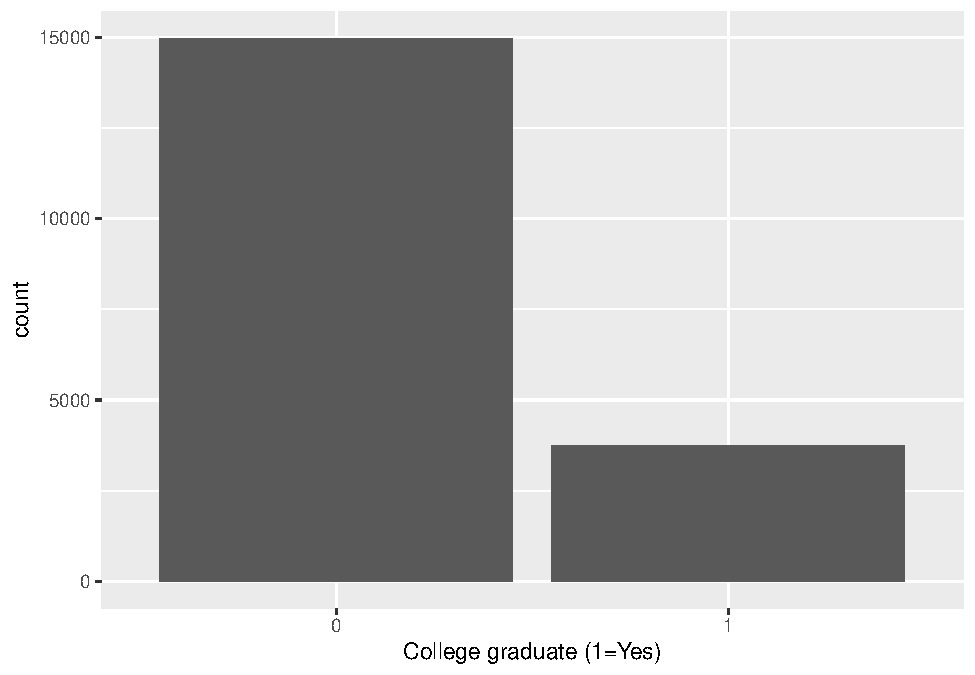
\includegraphics{RIntro_files/figure-latex/unnamed-chunk-24-1.pdf}

\hypertarget{continuous-variable-distributions}{%
\subsection{8.3. Continuous Variable
Distributions}\label{continuous-variable-distributions}}

\begin{Shaded}
\begin{Highlighting}[]
\FunctionTok{ggplot}\NormalTok{(}\AttributeTok{data =}\NormalTok{ nlswork\_no\_na) }\SpecialCharTok{+} \FunctionTok{geom\_histogram}\NormalTok{(}\AttributeTok{mapping =} \FunctionTok{aes}\NormalTok{(}\AttributeTok{x =}\NormalTok{ age), }\AttributeTok{binwidth =} \DecValTok{1}\NormalTok{) }\SpecialCharTok{+} 
  \FunctionTok{scale\_x\_continuous}\NormalTok{(}\AttributeTok{breaks =} \FunctionTok{seq}\NormalTok{(}\DecValTok{20}\NormalTok{, }\DecValTok{50}\NormalTok{, }\AttributeTok{by =} \DecValTok{5}\NormalTok{))}
\end{Highlighting}
\end{Shaded}

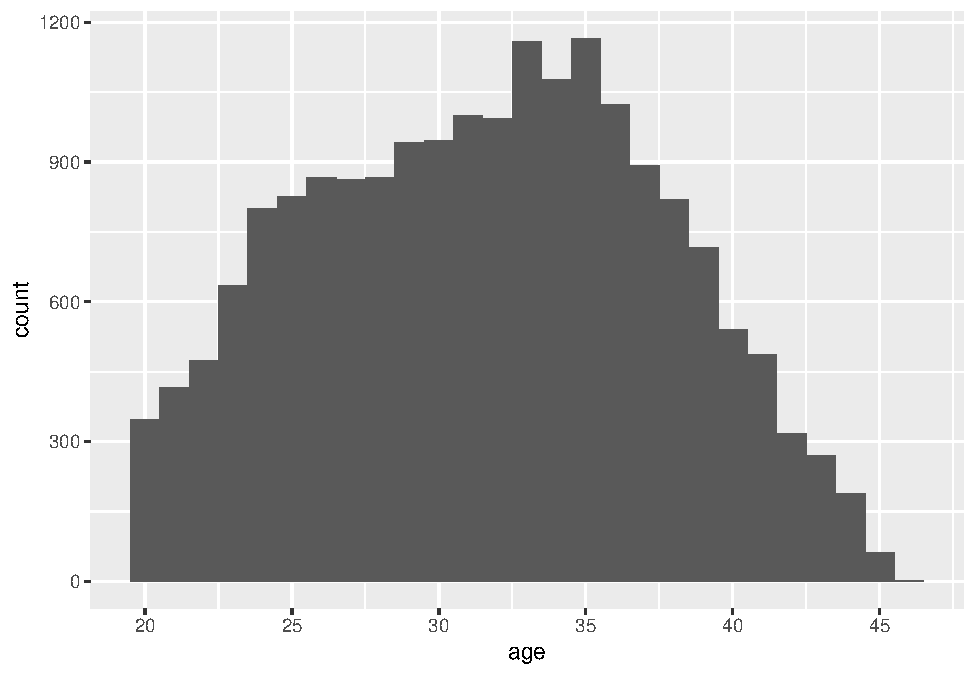
\includegraphics{RIntro_files/figure-latex/unnamed-chunk-25-1.pdf}

\hypertarget{categorical-and-continuous-variables}{%
\subsection{8.4 Categorical and continuous
variables}\label{categorical-and-continuous-variables}}

\begin{Shaded}
\begin{Highlighting}[]
\NormalTok{nlswork\_no\_na }\SpecialCharTok{\%\textgreater{}\%} \FunctionTok{ggplot}\NormalTok{(}\FunctionTok{aes}\NormalTok{(}\AttributeTok{x=}\FunctionTok{as.factor}\NormalTok{(collgrad), }\AttributeTok{y=}\NormalTok{ln\_wage\_winsorized)) }\SpecialCharTok{+}
  \FunctionTok{geom\_boxplot}\NormalTok{(}\AttributeTok{fill=}\StringTok{"slateblue"}\NormalTok{, }\AttributeTok{alpha=}\FloatTok{0.2}\NormalTok{) }\SpecialCharTok{+} 
  \FunctionTok{xlab}\NormalTok{(}\StringTok{"College graduate (1=Yes)"}\NormalTok{)}
\end{Highlighting}
\end{Shaded}

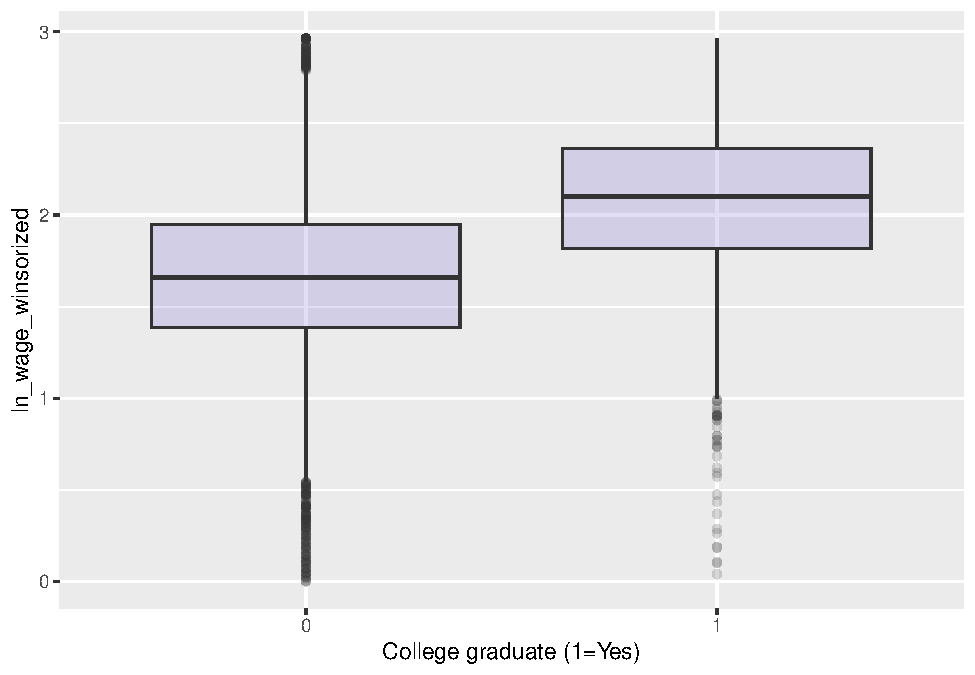
\includegraphics{RIntro_files/figure-latex/unnamed-chunk-26-1.pdf}

\begin{Shaded}
\begin{Highlighting}[]
\NormalTok{nlswork\_no\_na }\SpecialCharTok{\%\textgreater{}\%} \FunctionTok{ggplot}\NormalTok{(}\AttributeTok{mapping =} \FunctionTok{aes}\NormalTok{(}\AttributeTok{x =}\NormalTok{ ln\_wage, }\AttributeTok{y =}\NormalTok{ ..density..)) }\SpecialCharTok{+}
    \FunctionTok{xlab}\NormalTok{(}\StringTok{"ln(wage)"}\NormalTok{) }\SpecialCharTok{+}
    \FunctionTok{ylab}\NormalTok{(}\StringTok{"Density"}\NormalTok{) }\SpecialCharTok{+}
    \FunctionTok{geom\_freqpoly}\NormalTok{(}\AttributeTok{mapping =} \FunctionTok{aes}\NormalTok{(}\AttributeTok{colour =} \FunctionTok{factor}\NormalTok{(collgrad, }\AttributeTok{labels=}\FunctionTok{c}\NormalTok{(}\StringTok{"No"}\NormalTok{, }\StringTok{"Yes"}\NormalTok{)))) }\SpecialCharTok{+}
  \FunctionTok{labs}\NormalTok{(}\AttributeTok{color =}\StringTok{"College degree"}\NormalTok{)}
\end{Highlighting}
\end{Shaded}

\begin{verbatim}
## `stat_bin()` using `bins = 30`. Pick better value with `binwidth`.
\end{verbatim}

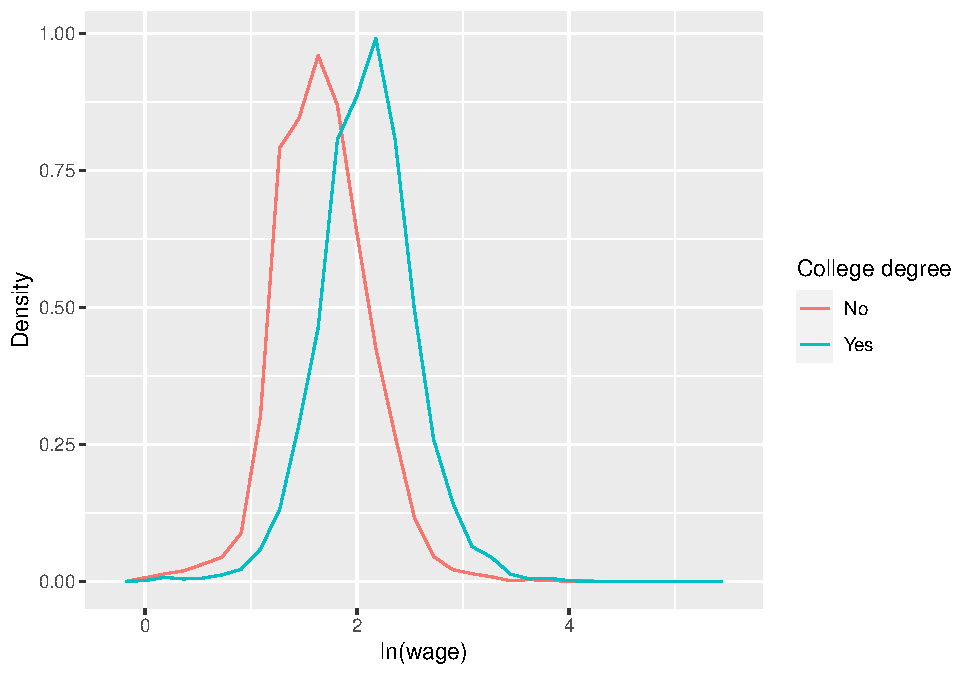
\includegraphics{RIntro_files/figure-latex/unnamed-chunk-27-1.pdf}

\hypertarget{correlation}{%
\section{9. Correlation}\label{correlation}}

\begin{Shaded}
\begin{Highlighting}[]
\FunctionTok{ggpairs}\NormalTok{(nlswork\_no\_na[, }\FunctionTok{c}\NormalTok{(}\StringTok{"age"}\NormalTok{,}\StringTok{"ttl\_exp"}\NormalTok{,}\StringTok{"hours"}\NormalTok{)], }\AttributeTok{title=}\StringTok{"Correlogram with ggpairs()"}\NormalTok{)}
\end{Highlighting}
\end{Shaded}

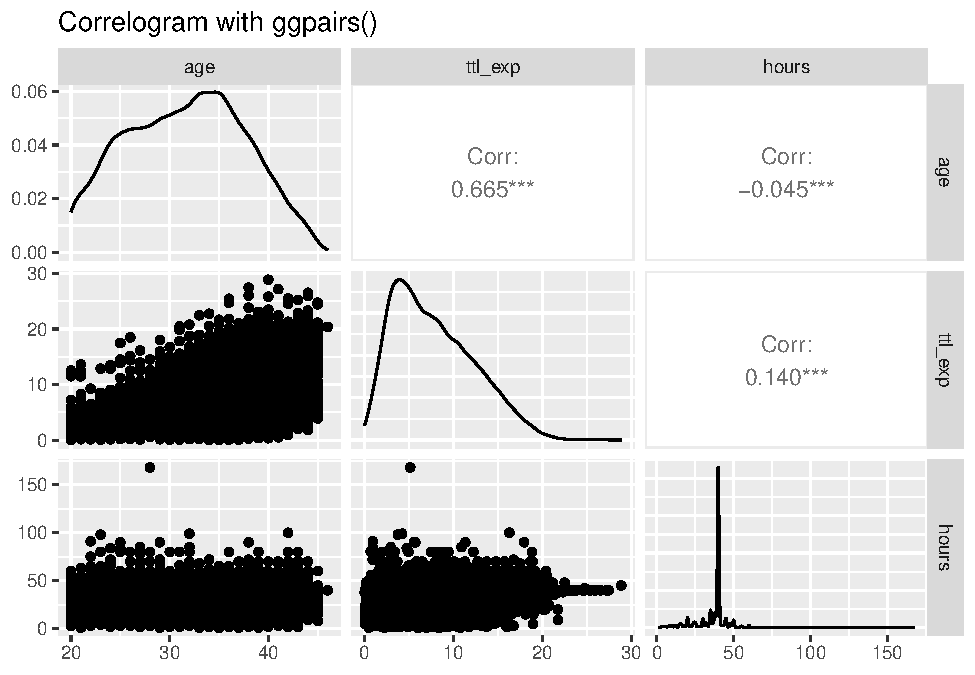
\includegraphics{RIntro_files/figure-latex/unnamed-chunk-28-1.pdf}

\hypertarget{assessment}{%
\section{10. Assessment}\label{assessment}}

\hypertarget{problem-1-data-importing}{%
\subsection{Problem 1: Data Importing}\label{problem-1-data-importing}}

Import the ``card'' dataset.

\begin{Shaded}
\begin{Highlighting}[]
\CommentTok{\#}\RegionMarkerTok{BEGIN}\CommentTok{ SOLUTION}
\NormalTok{card }\OtherTok{\textless{}{-}} \FunctionTok{as.data.frame}\NormalTok{(}\FunctionTok{read\_excel}\NormalTok{(}\StringTok{"card.xlsx"}\NormalTok{))}

\CommentTok{\#}\RegionMarkerTok{END}\CommentTok{ SOLUTION}
\end{Highlighting}
\end{Shaded}

\hypertarget{problem-2-visualizing-missing-data}{%
\subsection{Problem 2: Visualizing Missing
Data}\label{problem-2-visualizing-missing-data}}

Graphically show which variables have the most missing values. Please
elaborate.

\begin{Shaded}
\begin{Highlighting}[]
\CommentTok{\#}\RegionMarkerTok{BEGIN}\CommentTok{ SOLUTION}

\CommentTok{\#}\RegionMarkerTok{END}\CommentTok{ SOLUTION}
\end{Highlighting}
\end{Shaded}

\hypertarget{problem-3-handling-missing-data}{%
\subsection{Problem 3: Handling Missing
Data}\label{problem-3-handling-missing-data}}

Adopt a strategy to handle the missing values. Why did you follow that
strategy? How many observations were lost?

\begin{Shaded}
\begin{Highlighting}[]
\CommentTok{\#}\RegionMarkerTok{BEGIN}\CommentTok{ SOLUTION}

\CommentTok{\#}\RegionMarkerTok{END}\CommentTok{ SOLUTION}
\end{Highlighting}
\end{Shaded}

\hypertarget{problem-4-detecting-outliers}{%
\subsection{Problem 4: Detecting
outliers}\label{problem-4-detecting-outliers}}

Analyze if the variable lwage has outliers. If so, how will you deal
with them? Explain step by step.

\begin{Shaded}
\begin{Highlighting}[]
\CommentTok{\#}\RegionMarkerTok{BEGIN}\CommentTok{ SOLUTION}


\CommentTok{\#}\RegionMarkerTok{END}\CommentTok{ SOLUTION}
\end{Highlighting}
\end{Shaded}

\hypertarget{problem-5-descriptive-statistics-after-missing-data-and-outliers-handling}{%
\subsection{Problem 5: Descriptive Statistics after Missing Data and
Outliers
Handling}\label{problem-5-descriptive-statistics-after-missing-data-and-outliers-handling}}

Present statistics of the dataset that has been treated for missing
values and outliers.

\begin{Shaded}
\begin{Highlighting}[]
\CommentTok{\#}\RegionMarkerTok{BEGIN}\CommentTok{ SOLUTION}
\NormalTok{card\_media }\OtherTok{\textless{}{-}}\NormalTok{ card }\SpecialCharTok{\%\textgreater{}\%}
  \FunctionTok{mutate}\NormalTok{(}\FunctionTok{across}\NormalTok{(}\FunctionTok{c}\NormalTok{(}\StringTok{"IQ"}\NormalTok{, }\StringTok{"fatheduc"}\NormalTok{, }\StringTok{"motheduc"}\NormalTok{, }\StringTok{"KWW"}\NormalTok{, }\StringTok{"married"}\NormalTok{, }\StringTok{"libcrd14"}\NormalTok{),}
                \SpecialCharTok{\textasciitilde{}} \FunctionTok{ifelse}\NormalTok{(}\FunctionTok{is.na}\NormalTok{(.), }\FunctionTok{mean}\NormalTok{(., }\AttributeTok{na.rm =} \ConstantTok{TRUE}\NormalTok{), .))) }

\NormalTok{nlswork\_filled }\OtherTok{\textless{}{-}}\NormalTok{ nlswork }\SpecialCharTok{\%\textgreater{}\%} 
  \FunctionTok{mutate}\NormalTok{(}\FunctionTok{across}\NormalTok{(}\FunctionTok{c}\NormalTok{(}\StringTok{"union"}\NormalTok{), }\SpecialCharTok{\textasciitilde{}} \FunctionTok{ifelse}\NormalTok{(}\FunctionTok{is.na}\NormalTok{(.), }\FunctionTok{mean}\NormalTok{(., }\AttributeTok{na.rm =} \ConstantTok{TRUE}\NormalTok{), .))) }

\CommentTok{\#}\RegionMarkerTok{END}\CommentTok{ SOLUTION}
\end{Highlighting}
\end{Shaded}

\hypertarget{problem-6-relationship-visualization}{%
\subsection{Problem 6: Relationship
Visualization}\label{problem-6-relationship-visualization}}

Graphically show the relationship between age and salary.Does the
relationship between the variables make sense?

\begin{Shaded}
\begin{Highlighting}[]
\CommentTok{\#}\RegionMarkerTok{BEGIN}\CommentTok{ SOLUTION}

\CommentTok{\#}\RegionMarkerTok{END}\CommentTok{ SOLUTION}
\end{Highlighting}
\end{Shaded}

\hypertarget{problem-7-age-distribution}{%
\subsection{Problem 7: Age
Distribution}\label{problem-7-age-distribution}}

Display the distribution of Age

\begin{Shaded}
\begin{Highlighting}[]
\CommentTok{\#}\RegionMarkerTok{BEGIN}\CommentTok{ SOLUTION}

\CommentTok{\#}\RegionMarkerTok{END}\CommentTok{ SOLUTION}
\end{Highlighting}
\end{Shaded}

\hypertarget{problem-8-correlation}{%
\subsection{Problem 8: Correlation}\label{problem-8-correlation}}

What is the correlation value between age and salary?

\begin{Shaded}
\begin{Highlighting}[]
\CommentTok{\#}\RegionMarkerTok{BEGIN}\CommentTok{ SOLUTION}

\CommentTok{\#}\RegionMarkerTok{END}\CommentTok{ SOLUTION}
\end{Highlighting}
\end{Shaded}

\hypertarget{problem-9}{%
\subsection{Problem 9:}\label{problem-9}}

In the nlswork\_no\_na dataset, can you identify any patterns or trends
in the data related to unionized workers and their salaries?

\begin{Shaded}
\begin{Highlighting}[]
\CommentTok{\#}\RegionMarkerTok{BEGIN}\CommentTok{ SOLUTION}

\CommentTok{\#}\RegionMarkerTok{END}\CommentTok{ SOLUTION}
\end{Highlighting}
\end{Shaded}


\end{document}
